\documentclass[12pt]{article}

%environnement
\usepackage[letterpaper,margin=1in]{geometry}
\usepackage[utf8]{inputenc}
\usepackage{fontspec}
\usepackage[english]{babel}
\usepackage[parfill]{parskip}
\usepackage[style=ieee,backend=bibtex]{biblatex} %gestion bib
\usepackage{listings}
\usepackage{hyperref}
\usepackage[toc,acronym]{glossaries}
\usepackage[framemethod=TikZ]{mdframed} 
\usepackage{todonotes}
\usepackage[section]{placeins}
\hypersetup{
  pdftitle={},
  pdfborder={0 0 0}, %epaisseur box
  pdfauthor={Thomas LUINAUD},
}
\usepackage{tikz,tkz-tab}%package pour les tableaux de variations et de signes%
\usetikzlibrary{babel}
\usepackage{modules/tikzNetwork}
\usepackage{circuitikz}
\usetikzlibrary{positioning, automata, graphs, trees, fit, arrows.meta, shapes}
\usetikzlibrary{backgrounds,patterns,matrix,calc,shadows,plotmarks, circuits.logic.US}
\usetikzlibrary{decorations}
\usepackage{multirow}
\usepackage{modules/moeptikz}
%\usepackage{tabularx}
 %this file contains shape declaration and macro that define 
 %basic computer science shape for Hardware design.
 %this file should be include in the preamble
 
 \catcode`@=11

\pgfkeys{%
  /pgf/logicalbloc io north/.initial=5,
%  /pgf/logicalbloc io south/.initial=10,
%  /pgf/logicalbloc io east/.initial=10,
  /pgf/logicalbloc io west/.initial=10,
  /pgf/logicalbloc io north spacing/.initial=0.15cm,
%  /pgf/logicalbloc io south spacing/.initial=0.25cm,
%  /pgf/logicalbloc io east spacing/.initial=0.25cm,
  /pgf/logicalbloc io west spacing/.initial=0.20cm
}
\def\maxpins{100}


%stdChip
\pgfdeclareshape{logicalbloc}{
	\savedanchor\centerpoint{% 
		\pgf@x=.5\wd\pgfnodeparttextbox%
		\pgf@y=.5\ht\pgfnodeparttextbox%
		\advance\pgf@y by-.5\dp\pgfnodeparttextbox%
	  }
	  \anchor{center}{\centerpoint}
	  
	  \saveddimen\height{%
		\pgfmathsetlength\pgf@x{(\pgfkeysvalueof{/pgf/logicalbloc io west}+1)*\pgfkeysvalueof{/pgf/logicalbloc io west spacing}}%
	  }
	  \saveddimen\width{%
		\pgfmathsetlength\pgf@y{(\pgfkeysvalueof{/pgf/logicalbloc io north}+1)*\pgfkeysvalueof{/pgf/logicalbloc io north spacing}}%
	  }
	  \saveddimen{\yspacing}{\pgfmathsetlength\pgf@x{\pgfkeysvalueof{/pgf/logicalbloc io west spacing}}}	  
	  \saveddimen{\xspacing}{\pgfmathsetlength\pgf@y{\pgfkeysvalueof{/pgf/logicalbloc io north  spacing}}}
	  
	  \backgroundpath{%
		\pgfpathrectanglecorners{\pgfpointadd{\centerpoint}{\genbottomleftpoint}}%
		{\pgfpointadd{\centerpoint}{\gentoprightpoint}}%
	  }
 

	  \pgfmathloop%
	  \ifnum\pgfmathcounter>\maxpins\relax% 
	  \else%
		% Need to expand \pgfmathcounter
		\edef\marshal{\noexpand\anchor{io east \pgfmathcounter}}%
		\expandafter\marshal\expandafter{\expandafter\chippinanchorright\expandafter{\pgfmathcounter}}%
	  \repeatpgfmathloop%
	  
	  \pgfmathloop%
	  \ifnum\pgfmathcounter>\maxpins\relax% 
	  \else%
		% Need to expand \pgfmathcounter
		\edef\marshal{\noexpand\anchor{io north \pgfmathcounter}}%
		\expandafter\marshal\expandafter{\expandafter\chippinanchorupper\expandafter{\pgfmathcounter}}%
	  \repeatpgfmathloop%
	  
	  \pgfmathloop%
	  \ifnum\pgfmathcounter>\maxpins\relax% 
	  \else%
		% Need to expand \pgfmathcounter
		\edef\marshal{\noexpand\anchor{io south \pgfmathcounter}}%
		\expandafter\marshal\expandafter{\expandafter\chippinanchorbottom\expandafter{\pgfmathcounter}}%
	  \repeatpgfmathloop%
	  
	  \pgfmathloop%
	  \ifnum\pgfmathcounter>\maxpins\relax% 
	  \else%
		% Need to expand \pgfmathcounter
		\edef\marshal{\noexpand\anchor{io west \pgfmathcounter}}%
		\expandafter\marshal\expandafter{\expandafter\chippinanchorleft\expandafter{\pgfmathcounter}}%
	  \repeatpgfmathloop%
}

\def\genbottomleftpoint{%
%	\pgfmathsetlength{pgf@xb}{(\pgfkeysvalueof{/pgf/logicalbloc io north}+1)*\pgfkeysvalueof{/pgf/logicalbloc io north spacing}}%
%	\pgfmathsetlength{pgf@yb}{(\pgfkeysvalueof{/pgf/logicalbloc io west}+1)*\pgfkeysvalueof{/pgf/logicalbloc io west spacing}}%
%	\setlength{\pgf@xa}{1cm}
%	\setlength{\pgf@ya}{1cm}
%	\if \pgf@xb<\pgf@xa
%		\if \pgf@yb<\pgf@ya
%			\pgfpoint{-0.5cm}{-0.5cm}
%		\else
%			\pgfpoint{-0.5cm}{-(\pgfkeysvalueof{/pgf/logicalbloc io west}+1)*\pgfkeysvalueof{/pgf/logicalbloc io west spacing}/2}
%		\fi
%	\else
%		\if \pgf@yb<\pgf@ya
%			\pgfpoint{-(\pgfkeysvalueof{/pgf/logicalbloc io north}+1)*\pgfkeysvalueof{/pgf/logicalbloc io north spacing}/2}{-0.5cm}
%		\else
			\pgfpoint{-((\pgfkeysvalueof{/pgf/logicalbloc io north}+1)*\pgfkeysvalueof{/pgf/logicalbloc io north spacing})/2}{-((\pgfkeysvalueof{/pgf/logicalbloc io west}+1)*\pgfkeysvalueof{/pgf/logicalbloc io west spacing})/2}
%		\fi
%	\fi
}
\def\gentoprightpoint{%
%	\if {\pgfkeysvalueof{/pgf/logicalbloc io west} < \pgfkeysvalueof{/pgf/logicalbloc io east}}
%		\setlength{\pgf@xc}{1cm}
%	\else
%		\setlength{\pgf@xc}{1cm}
%	\fi
%	\if
%		\setlength{\pgf@xc}{1cm}
%	\else
%		\setlength{\pgf@xc}{1cm}
%	\fi
%	\pgfmathsetlength{pgf@xb}{(\pgfkeysvalueof{/pgf/logicalbloc io north}+1)*\pgfkeysvalueof{/pgf/logicalbloc io north spacing}}%
%	\pgfmathsetlength{pgf@yb}{(\pgfkeysvalueof{/pgf/logicalbloc io west}+1)*\pgfkeysvalueof{/pgf/logicalbloc io west spacing}}%
%	\setlength{\pgf@xa}{1cm}
%	\setlength{\pgf@ya}{1cm}
%	\if \pgf@xb<\pgf@xa
%		\if \pgf@yb<\pgf@ya
%			\pgfpoint{0.5cm}{0.5cm}
%		\else
%			\pgfpoint{0.5cm}{(\pgfkeysvalueof{/pgf/logicalbloc io west}+1)*\pgfkeysvalueof{/pgf/logicalbloc io west spacing}/2}
%		\fi
%	\else
%		\if \pgf@yb<\pgf@ya
%			\pgfpoint{(\pgfkeysvalueof{/pgf/logicalbloc io north}+1)*\pgfkeysvalueof{/pgf/logicalbloc io north spacing}/2}{0.5cm}
%		\else
			\pgfpoint{((\pgfkeysvalueof{/pgf/logicalbloc io north}+1)*\pgfkeysvalueof{/pgf/logicalbloc io north spacing})/2}{((\pgfkeysvalueof{/pgf/logicalbloc io west}+1)*\pgfkeysvalueof{/pgf/logicalbloc io west spacing})/2}
%		\fi
%	\fi
}


\def\genpointbottom#1{
\pgfpoint{(\pgfkeysvalueof{/pgf/logicalbloc io north}+1)*\pgfkeysvalueof{/pgf/logicalbloc io north spacing}/2-#1*\xspacing}{-(\pgfkeysvalueof{/pgf/logicalbloc io west}+1)*\pgfkeysvalueof{/pgf/logicalbloc io west spacing}/2}
}

\def\chippinanchorbottom#1{%
	  % When this macro is called,
	  % \centerpoint, \height and \chipspacing will be defined.
	  %\pgfpointadd{\centerpoint}{\pgfpoint{\width/2-#1*\xspacing}{-\height/2}}%
	  \pgfpointadd{\centerpoint}{\genpointbottom{#1}}%
}

\def\genpointupper#1{
\pgfpoint{(\pgfkeysvalueof{/pgf/logicalbloc io north}+1)*\pgfkeysvalueof{/pgf/logicalbloc io north spacing}/2-#1*\xspacing}{(\pgfkeysvalueof{/pgf/logicalbloc io west}+1)*\pgfkeysvalueof{/pgf/logicalbloc io west spacing}/2}
}

\def\chippinanchorupper#1{%
	  % When this macro is called,
	  % \centerpoint, \height and \chipspacing will be defined.
	  \pgfpointadd{\centerpoint}{\genpointupper{#1}}%
}

\def\genpointleft#1{
\pgfpoint{-(\pgfkeysvalueof{/pgf/logicalbloc io north}+1)*\pgfkeysvalueof{/pgf/logicalbloc io north spacing}/2}{(\pgfkeysvalueof{/pgf/logicalbloc io west}+1)*\pgfkeysvalueof{/pgf/logicalbloc io west spacing}/2-#1*\yspacing}
}

\def\chippinanchorleft#1{%
	  % When this macro is called,
	  % \centerpoint, \height and \chipspacing will be defined.
	  \pgfpointadd{\centerpoint}{\genpointleft{#1}}%
}

\def\genpointright#1{
\pgfpoint{(\pgfkeysvalueof{/pgf/logicalbloc io north}+1)*\pgfkeysvalueof{/pgf/logicalbloc io north spacing}/2}{(\pgfkeysvalueof{/pgf/logicalbloc io west}+1)*\pgfkeysvalueof{/pgf/logicalbloc io west spacing}/2-#1*\yspacing}
}
\def\chippinanchorright#1{%
	  % When this macro is called,
	  % \centerpoint, \height and \chipspacing will be defined.
	  \pgfpointadd{\centerpoint}{\genpointright{#1}}%
}

\catcode`@=12
\usepackage{cancel}%package pour barrer et simplifier%
\usepackage{amsmath}%matrice%
\usepackage{stmaryrd}
\usepackage{textcomp}
\usepackage{pstricks}
\usepackage{pdftricks, pstricks-add}
\usepackage{pgfplots}
\usepackage{caption}
\usepackage{subfig}
\usepackage{pdfpages}
	
\hyphenation{contien-nent}

\usepackage[nounderscore]{syntax}
\newlength\grammarLongest
\newlength\grammarLeftMargin
\makeatletter
\newenvironment{grammarC}[1]{%
\list{}{%
\settowidth\grammarLongest{#1}
\setlength\grammarLeftMargin{\dimexpr0.5\linewidth-0.5\grammarLongest}
\labelwidth\grammarindent%
\leftmargin\dimexpr\grammarindent+\grammarLeftMargin\relax%
\advance\grammarindent\labelsep
\itemindent\z@%
\listparindent\z@%
\parsep\grammarparsep%
}%
\let\\\@normalcr
\syntaxShortcuts\relax\relax%
\def\alt{\\\llap{\textbar\quad}}%
\def\gr@setpar{%
\def\par{%
\parshape\@ne\@totalleftmargin\linewidth%
\@@par%
\catcode`\<12%
\everypar{%
\everypar{}%
\catcode`\<\active%
\gr@implitem%
}%
}%
}%
\gr@setpar%
\par%
\let\gr@leftsq\[%
\let\gr@rightsq\]%
\def\gr@endsyntdiag]{\end{syntdiag}\gr@setpar\par}%
\def\[{\@ifnextchar[{\begin{syntdiag}\@gobble}\gr@leftsq}%
\def\]{\@ifnextchar]\gr@endsyntdiag\gr@rightsq}%
}{%
\@newlistfalse%
\everypar{}%
\endlist%
}
\makeatother
\usepackage{varwidth}

\usepackage{tabularx}
\usepackage{csvsimple}
\usepackage{float}
\usepackage{amssymb}
\usepackage[linesnumbered,lined, french, frenchkw, figure, noend]{algorithm2e}

\newcommand{\inputFig}[2]{\IfFileExists{#1}{\input{#1}}{\missingfigure[figheight=3cm]{#2}}}

\newsavebox{\tempbox}
\newsavebox{\tempboxi}


% Title Page
\title{Rapport de l'étape 1 du projet compilateur \\ Étape 1}
\author{Francis de Ladurantaye \\ Thomas Luinaud}


\begin{document}
\begin{titlepage}
  \maketitle
\end{titlepage}

\section{Structure logicielle}
\begin{figure}[h]
	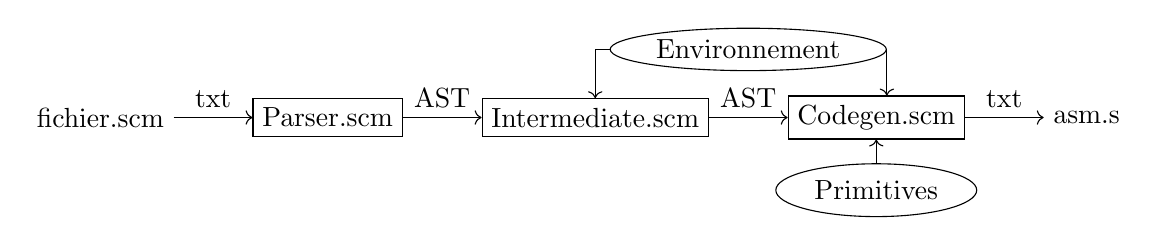
\begin{tikzpicture}
		\node[](file) {fichier.scm};
		\node[draw, right=of file] (parser) {Parser.scm};
		\node[draw, right=of parser] (intermediate) {Intermediate.scm};
		\node[draw, right=of intermediate] (codegen) {Codegen.scm};
		\node[right=of codegen] (asm) {asm.s};
		\node[below =0.3cm of codegen,ellipse, draw](prims) {Primitives};
		
		\path[draw, ->] (prims) -- (codegen);
		\path[->] (file) edge node [above] {txt} (parser)
				  (parser) edge node [above] {AST} (intermediate)
				  (intermediate) edge node (outIR)  [above] {AST} (codegen)
				  (codegen) edge node [above] {txt} (asm);
		\node[above =0.1cm of outIR, ellipse, draw, inner sep=2pt](symbTable) {Environnement};
		\path[draw, ->] (symbTable) -| (intermediate);
		\path[draw, ->] (symbTable) -| (codegen.north -| symbTable.east);
	\end{tikzpicture}
	\caption{structure du compilateur}
\end{figure}

\newpage
\section{ancien rapport}
\section{Spécification du problème}
Le but du projet est de réaliser un compilateur pour un sous-ensemble sélectionné du langage de programmation Scheme. Le travail à réaliser étant divisé en trois étapes, nous devrons chaque fois étendre notre support à un plus grand sous-ensemble du langage, en construisant à partir du point où nous nous étions arrêté lors de l'étape précédente. À terme, le compilateur résultant devra être autogène, c'est-à-dire d'être en mesure de se compiler lui-même, de façon à garantir son autosuffisance en éliminant les dépendances aux compilateurs Scheme existants. Cela implique inévitablement que le sous-ensemble que nous chercherons à supporter au terme de la troisième étape devra être suffisamment étendu afin d'offrir la puissance nécessaire à l'atteinte de cet objectif mais également d'écrire le compilateur en prenant en compte les éléments que nous supporterons.

\subsection{Sous-ensemble de Scheme à supporter}
Au terme de l'étape 1 du projet, il est attendu de nous que le parseur produit soit habilité à supporter les constructions syntaxiques suivantes :

\begin{itemize}
\item Nombres entiers positifs et négatifs
\item Booléens \texttt{\#t} et \texttt{\#f}
\item Caractères, qui débutent par \texttt{\#\textbackslash}
\item Chaînes de caractères et caractère d'échappement ``\texttt{\textbackslash}"
\item Symboles
\item Listes propres et impropres
\item Commentaires
\end{itemize}

De son côté, le générateur de code devra permettre la compilation des expressions suivantes en se limitant pour l'instant simplement à la manipulation d'entiers et de booléens :

\begin{itemize}
\item Constantes entières
\item Constantes booléennes
\item \texttt{(println} $expr$\texttt{)}
\item \texttt{(+} $expr_1$ $expr_2$\texttt{)}
\item \texttt{(-} $expr_1$ $expr_2$\texttt{)}
\item \texttt{(*} $expr_1$ $expr_2$\texttt{)}
\item \texttt{(quotient} $expr_1$ $expr_2$\texttt{)}
\item \texttt{(modulo} $expr_1$ $expr_2$\texttt{)}
\item \texttt{(=} $expr_1$ $expr_2$\texttt{)}
\item \texttt{(<} $expr_1$ $expr_2$\texttt{)}
\item \texttt{(if} $expr_1$ $expr_2$ $expr_3$\texttt{)}
\item \texttt{(let ((}$var_1$ $expr_1$\texttt{) ...)} $expr_0$\texttt{)}
\end{itemize}

\subsection{Analyseur lexical (parseur)}
En ce qui concerne la première étape du projet, il nous était demandé d'être en mesure de compiler et exécuter des fichiers Scheme simples ne comportant que les constructions syntaxiques du sous-ensemble de Scheme à supporter pour le moment. Cela implique que notre compilateur doit inclure un analyseur lexical (parseur) et syntaxique (générateur de code) utilisant l'approche par descente récursive, dont les rôles seront respectivement d'effectuer la lecture des fichiers à compiler, caractère par caractère, afin d'en extraire les différents éléments et de produire le code machine résultant. En plus d'extraire les éléments pertinents lors de se traversée (lecture), le parseur doit aussi effectuer le regroupement des éléments extraits en expressions (listing), simplifiant ainsi le travail du générateur de code assembleur qui n'aura donc nul besoin de retraverser ces fichiers à la suite du parseur.

Afin d'illustrer le travail du parseur, supposons que le contenu du fichier à compiler est le suivant : "Hello World!". Le parseur, lors de sa traversée dudit fichier, reconnaîtra le guillemet se trouvant au début et, sachant alors qu'il se trouve dans une chaîne de caractères, lira successivement les caractères suivants jusqu'à ce qu'il tombe sur le guillemet fermant à la suite duquel cet élément \textit{chaîne de caractère} sera ajouté à une liste servant à représenter le sens du programme. Cette étape est très importante car, dans le cas présent, le caractère d'espacement au centre de la chaîne n'a ici pas d'autre sens que celui d'un simple caractère, mais il aurait signifié la délimitation entre deux éléments distincts s'il ne s'était pas trouvé entouré d'une paire de guillemets. De nombreux caractères ayant ainsi plusieurs sens, et ce dans tous les langages de programmation, un générateur de code devant effectuer cette tâche parallèlement à la production du code machine paraît quasi irréalisable, l'implantation d'un simple parseur représentant déjà un défi non négligeable.

\subsection{Analyseur syntaxique (générateur de code)}
Le générateur de code est l'élément central du compilateur. Une fois produit le \textit{listing} des expressions, le générateur de code a tout ce dont il a besoin pour effectuer sa tâche. Cela s'explique par le fait que la représentation sous forme de \textit{listing} des expressions du programme correspond au sens de celui-ci, de manière dissociée de la chaîne de caractères dont il provient. Le travaille du générateur de code se résume donc à parcourir le listing reçu et d'en traiter les éléments de la façon appropriée, ce pour en générer le code machine dont l'exécution produira les résultats correspondant au programme originel.

Cette tâche est cependant plus compliquée qu'il n'y paraît. En effet, le générateur se charge non seulement de la génération de code, mais aussi de s'assurer que les expressions reçues sont syntaxiquement correctes. Cela nécessite entre autres de vérifier que les procédures contenues dans les expressions ont le nombre d'arguments attendu ou que les variables apparaissant dans les expressions ont bien été initialisées antérieurement à leur utilisation. En outre, c'est au générateur de code qu'il revient de gérer les fermetures lors de la présence de \texttt{let} et de s'assurer que l'accès au contenu d'une variable ayant ainsi été redéfinie renvoie la valeur attendue. Ces difficultés ne font que s'accumuler lorsque le programme à compiler contient de multiples \texttt{let} imbriqués, requérant une gestion de la pile appropriée à ces constructions syntaxiques qui sont tout à fait correctes.

Comme dernières complications liées au générateur de code assembleur, la gestion des symboles et des énoncés conditionnels. Au niveau de l'énoncé conditionnel \texttt{if}, la génération des étiquettes servant à sauter les blocs ne devant pas être exécutés doit être gérée de façon particulière car plusieurs \texttt{if} peuvent se trouver dans un même programme. Il est important que chacun d'eux n'effectue pas de saut vers des portions de code des autres \texttt{if}. En lien direct avec les énoncés conditionnels, certains symboles sont particulièrement importants. Nous parlons bien entendu ici des symboles \texttt{\#t} et \texttt{\#f} qui doivent être reconnus par le générateur de code car, ne se trouvant pas dans l'environnement comme ceux associés aux variables ou référant à des procédures, une recherche dans l'environnement engendrerait la détection d'une variable non initialisée.

Toutes ces difficultés seront donc à prendre en considération tout au long de l'implémentation du générateur de code afin de s'éviter d'avoir de mauvaises surprises nécessitant de recoder le corps de plusieurs fonctions, et ce possiblement à de multiples occasions.

\subsection{Tests unitaires}
Enfin, le dernier élément du travail à réaliser était la conception de tests unitaires pertinents servant à vérifier le bon fonctionnement des différents éléments de notre compilateur, principalement du parseur et du générateur de code. En plus des 27 tests fournis, nous devions en produire entre 30 et 50 tests supplémentaires pour bien vérifier chaque fonctionnalité. Les résultats des tests seront présentés dans une section subséquente de ce rapport.


\section{Méthodologie}
En ce qui a trait à la méthodologie adoptée pour l'attente des objectifs, nous avons débuté par l'analyse des fichiers fournis afin de nous faire une certaine idée de la direction dans laquelle nous lancer. Nous avons testé de façon extensive la fonction \texttt{read} afin de bien comprendre ce qui était attendu comme résultat de la traversée d'un fichier par notre futur parseur. Ce faisant, nous avons aussi constaté les manques de cette fonction, nous donnant donc une idée assez claire sur ce qu'il restait à y implémenter.

Autrement, nous avons testé les différentes commandes offertes par le \texttt{makefile} fourni, ce qui nous permit rapidement de comprendre comment lancer le compilateur pour exécuter les tests unitaires. Nous avons donc rapidement pu écrire des tests supplémentaires, ce qui nous aida grandement au débogage lorsque nous tentions d'implanter de nouvelles fonctionnalités et encore plus grandement lorsqu'il nous était nécessaire de réimplémenter une fonction après avoir constaté un problème.

Par ailleurs, nous nous sommes fréquemment référé à la documentation du langage Scheme telle que présentée dans les fichiers PDF \texttt{r5rs.pdf} et \texttt{r7rs.pdf} que nous avons téléversé sur notre répertoire GitHub. Bien que nous n'ayons pas suivi à la lettre ce que nous y avons lu sur la structure lexicale et la représentation externe du langage, cette documentation nous a grandement guidés lors de la construction de notre grammaire pour l'implantation de la fonction \texttt{read} de notre parseur.

Du côté de la gestion du répertoire GitHub, nous avons tenté d'effectuer nos changements sur des branches séparées de la branche principale afin de conserver la branche \textit{master} dans un état fonctionnel, mais nous avons tout de même dû revenir à un état antérieur à un certain point comme nous avions tenté d'adopter une nouvelle philosophie pour le parseur qui ne s'est finalement pas révélée viable.

\section{Problèmes rencontrés}

\subsection{Symboles \texttt{\#t} et \texttt{\#f}}
Parmi les problèmes rencontrés, les plus notables se sont révélés être la gestion des symboles \texttt{\#t} et \texttt{\#f}, de la forme spéciale \texttt{let} et des listes impropres. Concernant la reconnaissance des symboles \texttt{\#t} et \texttt{\#f}, la difficulté fut de se rendre compte que le symbole retourné par \texttt{(string->symbol "\#f")} était \texttt{|\#f|} et non pas \texttt{'\#f} et qu'il fallait donc explicitement retourner \texttt{'\#f} en présence de la chaîne \texttt{"\#f"}. Nous saurons donc à l'avenir que dans le langage Scheme, l'expression \texttt{string->symbol} ajoute une barre verticale de chaque côté du symbole résultant lorsque la chaîne à convertir débute par les caractères \texttt{\#} ou \texttt{\textbackslash}.

\subsection{Forme spéciale \texttt{let}}
La gestion de la forme spéciale \texttt{let}, nous l'affirmons avec grande conviction, fut la plus difficile à implémenter. Nous avions initialement prévu ajouter les variables qui y sont définies, accompagnées de leur valeur, dans une liste d'association représentant l'environnement, mais nous nous sommes rapidement rendu compte que cela ne permettrait pas d'accéder aux valeurs de ces variables une fois le code compilé vers l'assembleur. Ce pour quoi nous avons opté a été de garder dans l'environnement les variables déclarées au sein du  \texttt{let}, mais plutôt que de les y mettre avec leurs valeurs, nous les y avons mises accompagnées du décalage à effectuer par rapport au dessous de la pile pour retrouver leur valeur sur la pile. Ainsi, lors d'un accès à ces variables, la première étape consiste à retrouver le décalage dans l'environnement d'évaluation, puis à retrouver la valeur de cette variable dans la pile. De plus, en conservant dans le registre \texttt{\%rbp} la valeur de \texttt{\%rsp} au premier\texttt{let} rencontré, cela nous permet d'aisément gérer un nombre arbitraire de \texttt{let} imbriqués en n'ayant aucune difficulté.

Les autres difficultés rencontrées lors de l'implémentation de la forme spéciale \texttt{let} furent celle de restaurer l'environnement à son état initial à la sortie et le fait qu'il faille évaluer chacune des expressions avant de commencer à assigner les résultats aux variables à lier. Pour ce faire, nous avons commencé par garder dans des variables (\texttt{old-env} et \texttt{old-stack}) l'état de l'environnement et du décalage par rapport au dessous de la pile avant d'étendre l'environnement avec les nouvelles affectations; cela nous permettant de pouvoir effectuer la restauration à la sortie. Ensuite, nous effectuons le calcul de l'expression dont le résultat sera affecté à la première variable. Toutefois, plutôt que d'immédiatement mettre la variable dans l'environnement (avec son décalage dans la pile), nous allons plutôt récursivement faire de même avec toutes les autres expressions à calculer pour les liaisons. C'est seulement une fois toutes ces expressions évaluées que nous regroupons toutes les variables avec leur décalage sur la pile et que nous les utilisons pour étendre l'environnement. C'est donc de cette façon que nous arrivons à respecter le comportement que doit avoir la forme spéciale \texttt{let} en Scheme.

\subsection{Listes impropres}
Bien que les listes propres ne nous aient causé aucun problème, il n'en fut point de même quant à la gestion des listes impropres. La structure même des listes impropres a été ce qui nous a causé le plus de problèmes, celles-ci ne devant pas débuter ni terminer par le point signifiant l'impropreté de la liste. Nous avons donc dû, au sein du parseur, ajouter deux fonctions supplémentaires pour la lecture des listes, l'une faisant office de point d'entrée afin de s'assurer que la liste ne début pas par le point, l'autre faisant office de point de sortie (nécessaire seulement dans le cas d'une liste impropre) afin de s'assurer que le point ne termine pas non plus la liste. Nous sommes toutefois satisfaits de la façon dont nous sommes arrivés à gérer cela et trouvons finalement le résultat assez propre.


\section{Résultats des tests unitaires}
Tous les tests fournis pour l'étape 1 fonctionnent à merveille. De plus, les tests que nous avons conçus pour tester les différentes fonctionnalités passent non seulement correctement lors du \texttt{make ut}, ils nous ont aussi été d'une grande aide tout au long du développement de notre compilateur. Comme vous pourrez le constater, certains tests unitaires échouent malgré ce qui vient d'être mentionné, mais ces échecs sont normaux au point où nous en sommes. En effet, certains d'entre eux visent à tester le parseur alors que les expressions qu'ils contiennent ne sont pas encore supportées au niveau de la génération de code, expliquant que les erreurs surviennent uniquement dans le fichier \texttt{codegen.scm} et non pas dans \texttt{parser.scm}. C'est le cas par exemple des tests suivants, qui testent le parseur sur les chaînes de caractères, la quotation et les listes, propres et impropres :

\begin{itemize}
\item \texttt{let-string-println.scm}
\item \texttt{let-string-println-number.scm}
\item \texttt{list-impropre-comp.scm}
\item \texttt{list-proper1.scm}
\item \texttt{list-proper2.scm}
\item \texttt{list-proper-empty.scm}
\item \texttt{println-let-strings.scm}
\item \texttt{println-list-impropre1.scm}
\item \texttt{println-list-proper1.scm}
\item \texttt{println-quote.scm}
\item \texttt{println-string.scm}
\end{itemize}

De plus, nous avons aussi écrit des tests dont le but est d'échouer afin de nous assurer que des expressions invalides entraînent effectivement des erreurs. C'est le cas des tests qui débutent par \texttt{crash}, tels que les suivants :

\begin{itemize}
\item \texttt{crash-let.scm} $\rightarrow$ \texttt{let} sans \textit{body}
\item \texttt{crash-println-if-let-multi.scm} $\rightarrow$ contient l'expression \texttt{(\#t 156)}
\item \texttt{crash-quote-double.scm} $\rightarrow$ \texttt{quote} suivi de deux arguments
\item \texttt{crash-vide.scm} $\rightarrow$ liste vide sans quote (sans \texttt{'} au début)
\end{itemize}

\section{Atteinte des objectifs}
En conclusion, nous sommes très satisfaits du travail accompli. Au meilleur de nos connaissances, nous avons réussi à faire fonctionner complètement ce qui était demandé et avons même pris un peu d'avance sur les prochaines étapes. Nous avons hâte de voir comment gérer l'allocation dynamique de façon à pouvoir supporter le \texttt{define} et représenter les listes en mémoire.

Enfin, l'idée d'atteindre le stade où notre compilateur sera autogène nous anime et nous attendons impatiemment de voir les fonctionnalités supplémentaires que nous aurons à supporter au terme de la prochaine étape.

\newpage

\section{Annexes}

\subsection{Grammaire}
Voici notre grammaire (approximative et fortement inspiré de la documentation R7RS) pour l'implantation de notre parseur :
\begin{figure}[h!]
  %commande \alt permet de mettre une | en début de ligne pour continuer une expression en mettant un retour à la ligne
%grammarC permet de centrer le code le paramètre contient la plus longue ligne

\begin{grammarC}{<expression> ::= <expression-ent> | <opérateur> <entiers>}
  
  <datum> ::= <datum simple> | <procédure> | <abréviation>
  
  <abréviation> ::= <abrev> <datum>
  
  <abrev> ::= "'" | \space "\`" | ","
  
  <procédure> ::= ( <opérateur> <données> )
  
  <datum simple> ::= <booléen> | <nombre> | <symbole> | <string>
  
  <booléen> ::= \#t | \#f
  
  <string> ::= \verb|"| <element string>* \verb|"|
  
  <element string> ::= <tout caractère différent de \verb|" \|  > | \verb|\"| | \verb|\\|
  
  <opérateur> ::= "+" | "-" | "*" | "=" | "<" | <symbol>
  
  <nombre> ::= <valeurNeg> | <valeurPos>
  
  <valeurNeg> ::= "-" <entier>
  
  <valeurPos> ::= <signePos> <entier>
  
  <entier> ::= <digit> <entier> | <digit>
  
  <signePos> ::= "+" | $\epsilon$ 
  
  <digit> ::= '0' | '1' | '2' | '3' | '4' | '5' | '6' | '7' | '8' | '9'		
  
\end{grammarC}

  \caption{Représentation EBNF de la grammaire à supporter.}
\end{figure}

\end{document}          
